\documentclass[nobib]{tufte-handout}

%\\geometry{showframe}% for debugging purposes -- displays the margins

\newcommand{\bra}[1]{\left(#1\right)}
\usepackage{amssymb}
\usepackage{hyperref}
\usepackage[activate={true,nocompatibility},final,tracking=true,kerning=true,spacing=true,factor=1100,stretch=10,shrink=10]{microtype}
\usepackage{color}
\usepackage{steinmetz}
% Fixes captions and images being cut off
\usepackage{marginfix}
\usepackage{array}
\usepackage{tikz}
\usepackage{amsmath,amsthm}
\usetikzlibrary{shapes}
\usetikzlibrary{positioning}
\usepackage{listings}
\usepackage{caption}
\usepackage{circuitikz}
\DeclareCaptionFont{white}{\color{white}}
\DeclareCaptionFormat{listing}{\colorbox{gray}{\parbox{\textwidth}{#1#2#3}}}
\captionsetup[lstlisting]{format=listing,labelfont=white,textfont=white}

% Set up the images/graphics package
\usepackage{graphicx}
\setkeys{Gin}{width=\linewidth,totalheight=\textheight,keepaspectratio}
\graphicspath{{.}}

\title{Notes for ME27000 - Basic Mechanics I}
\author[Shubham Saluja Kumar Agarwal]{Shubham Saluja Kumar Agarwal}
\date{\today}  % if the \date{} command is left out, the current date will be used

\usepackage{pgfplots}
% The following package makes prettier tables.  We're all about the bling!
\usepackage{booktabs}

% The units package provides nice, non-stacked fractions and better spacing
% for units.
\usepackage{units}

% The fancyvrb package lets us customize the formatting of verbatim
% environments.  We use a slightly smaller font.
\usepackage{fancyvrb}
\fvset{fontsize=\normalsize}

% Small sections of multiple columns
\usepackage{multicol}

% For finite state machines 
\usetikzlibrary{automata} % Import library for drawing automata
\usetikzlibrary{positioning} % ...positioning nodes
\usetikzlibrary{arrows} % ...customizing arrows
\tikzset{node distance=2.5cm, % Minimum distance between two nodes. Change if necessary.
    every state/.style={ % Sets the properties for each state
    semithick,
    fill=gray!10},
    initial text={}, % No label on start arrow
    double distance=2pt, % Adjust appearance of accept states
    every edge/.style={ % Sets the properties for each transition
    draw,
    ->,>=stealth', % Makes edges directed with bold arrowheads
    auto,
    semithick}}
\let\epsilon\varepsilon

% These commands are used to pretty-print LaTeX commands
\newcommand{\doccmd}[1]{\texttt{\textbackslash#1}}% command name -- adds backslash automatically
\newcommand{\docopt}[1]{\ensuremath{\langle}\textrm{\textit{#1}}\ensuremath{\rangle}}% optional command argument
\newcommand{\docarg}[1]{\textrm{\textit{#1}}}% (required) command argument
\newenvironment{docspec}{\begin{quote}\noindent}{\end{quote}}% command specification environment
\newcommand{\docenv}[1]{\textsf{#1}}% environment name
\newcommand{\docpkg}[1]{\texttt{#1}}% package name
\newcommand{\doccls}[1]{\texttt{#1}}% document class name
\newcommand{\docclsopt}[1]{\texttt{#1}}% document class option name

% Define a custom command for definitions and biconditional
\newcommand{\defn}[2]{\noindent\textbf{#1}:\ #2}
\let\biconditional\leftrightarrow

\begin{document}

\maketitle

\begin{abstract}
    These are lecture notes for fall 2024 ME27000 at Purdue as taught by Professor Fabio Semperlotti. Modify, use, and distribute as you please.
\end{abstract}

\tableofcontents

\newpage

\section{Vectors, units, dimensions, significant digits}
\subsection{Vectors}
Two main types of quantities:
\begin{itemize}
    \item SCALAR: real value quantities
    \item VECTOR: defined by magnitude and direction.\\
    \begin{center}
        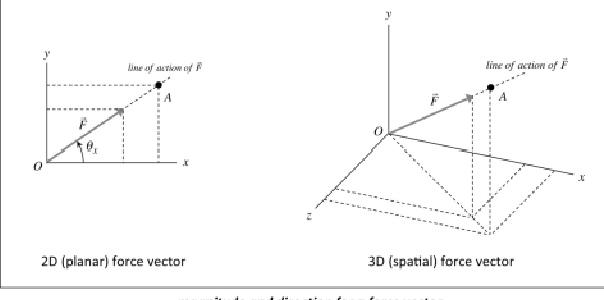
\includegraphics[width = 200px]{images/vector.png}
    \end{center}
\end{itemize}
There are also categories of vectors:
\begin{itemize}
    \item Fixed vector: the application point of the vector matters.
    \item Static vector: the application point of the vector can slide along the line of action to the same effect.
\end{itemize}

Most of the work in this course revolves around Newton's Laws, and their effects on and as vectors.
\subsection{Units and dimensions}
\defn{Dimension}{qualitative characterization of physical quantity, such as Force.}\\
\defn{Unit}{scale for a quantitative characterization of the physical quantity, such as Newton.}\\
The systems used for units are the SI, and British (imperial).
\subsection{Significant Digits}
The level of accuracy of numerical values dealt with in relevant mathematical operations.\\

\end{document}

